\chapter{Execution of a PASS Model}

\section{Informal Description of Subject Behavior and its Execution}
The excution of subject means sending and reveiving messages and executing internal activities in the defined order. In the following sections it is described what sending and receiving messages and executing internal functions means.

\subsection{Sending Messages}
Before sending a message, the values of the parameters to be transmitted need to be determined. In case the message parameters are simple data types, the required values are taken from local variables or business objects of the sending subject, respectively. In case of business objects, a current instance of a business object is transferred as a message parameter.\\
The sending subject attempts to send the message to the target subject and store it in its input pool. Depending on the described configuration and status of the input pool, the message is either immediately stored or the sending subject is blocked until a delivery of the message is possible.\\
In the sample business trip application, employees send completed requests using the message ‘send business trip request’ to the manager’s input pool. From a send state, several messages can be sent as an alternative. The following example shows a send state in which the message M1 is sent to the subject S1, or alternatively the message M2 is sent to S2, therefore referred to as alternative sending (see Figure \ref{fig:sendstate}). It does not matter which message is attempted to be sent first. If the send mechanism is successful, the corresponding state transition is executed. In case the message cannot be stored in the input pool of the target subject, sending is interrupted automatically, and another designated message is attempted to be sent. A sending subject will thus only be blocked if it cannot send any of the provided messages.

\begin{figure}[ph]
	\centering
	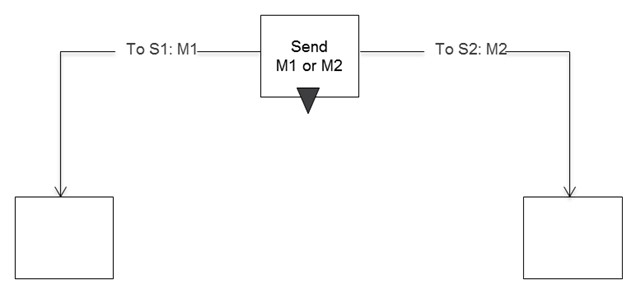
\includegraphics[width=0.7\linewidth]{20181026-Ontologie-Bilder/Grafiken-Ontologie/SUbjectExecution/sendState}
	\caption[Example of alternative sending]{Example of alternative sending}
	\label{fig:sendstate}
\end{figure}

By specifying priorities, the order of sending can be influenced. For example, it can be determined that the message M1 to S1 has a higher priority than the message M2 to S2. Using this specification, the sending subject starts with sending message M1 to S1 and then tries only in case of failure to send message M2 to S2. In case message M2 can also not be sent to the subject S2, the attempts to send start from the beginning.

The blocking of subjects when attempting to send can be monitored over time with the so-called timeout. The example in Figure \ref{fig:sendstatetimer} shows with ‘Timeout: 24 h’ an additional state transition which occurs when within 24 hours one of the two messages cannot be sent. If a value of zero is specified for the timeout, the process immediately follows the timeout path when the alternative message delivery fails completely.

\begin{figure*}[ph]
	\centering
	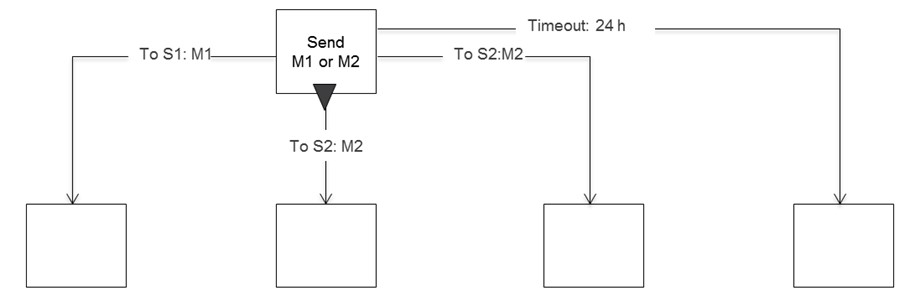
\includegraphics[width=0.7\linewidth]{20181026-Ontologie-Bilder/Grafiken-Ontologie/SUbjectExecution/SendSTateTimer}
	\caption[Send using time monitoring]{Send using time monitoring}
	\label{fig:sendstatetimer}
\end{figure*}


\subsection{Receiving Messages}
Analogously to sending, the receiving procedure is divided into two phases, which run inversely to send.

The first step is to verify whether the expected message is ready for being picked up. In case of synchronous messaging, it is checked whether the sending subject offers the message. In the asynchronous version, it is checked whether the message has already been stored in the input pool. If the expected message is accessible in either form, it is accepted, and in a second step, the corresponding state transition is performed. This leads to a takeover of the message parameters of the accepted message to local variables or business objects of the receiving subject. In case the expected message is not ready, the receiving subject is blocked until the message arrives and can be accepted.

In a certain state, a subject can expect alternatively multiple messages. In this case, it is checked whether any of these messages is available and can be accepted. The test sequence is arbitrary, unless message priorities are defined. In this case, an available message with the highest priority is accepted. However, all other messages remain available (e.g., in the input pool) and can be accepted in other receive states.

Figure \ref{fig:receivestate} shows a receive state of the subject ‘employee’ which is waiting for the answer regarding a business trip request. The answer may be an approval or a rejection.

\begin{figure}[ph]
	\centering
	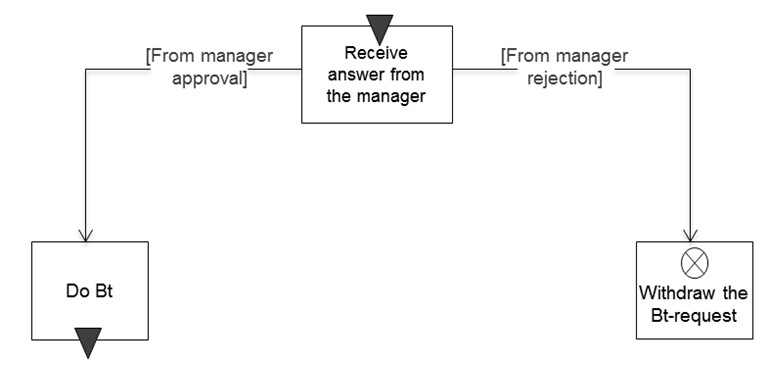
\includegraphics[width=0.7\linewidth]{20181026-Ontologie-Bilder/Grafiken-Ontologie/SUbjectExecution/ReceiveState}
	\caption[Example of alternative receiving]{Example of alternative receiving}
	\label{fig:receivestate}
\end{figure}

Just as with sending messages, also receiving messages can be monitored over time. If none of the expected messages are available and the receiving subject is therefore blocked, a time limit can be specified for blocking. After the specified time has elapsed, the subject will execute the transition as it is defined for the timeout period. The duration of the time limit may also be dynamic, in the sense that at the end of a process instance the process stakeholders assigned to the subject decide that the appropriate transition should be performed. We then speak of a manual timeout.

\begin{figure}[ph]
	\centering
	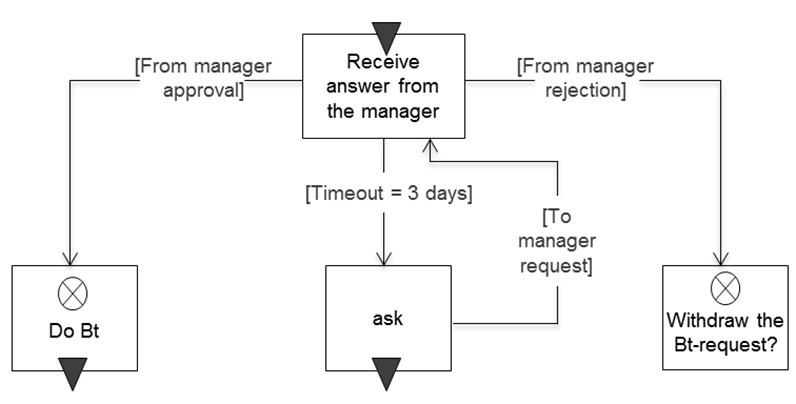
\includegraphics[width=0.7\linewidth]{20181026-Ontologie-Bilder/Grafiken-Ontologie/SUbjectExecution/ReceiveStateTimer}
	\caption[Time monitoring for message reception]{Time monitoring for message reception}
	\label{fig:receivestatetimer}
\end{figure}

\newpage
Figure \ref{fig:receivestatetimer} shows that, after waiting three days for the manager’s answer, the employee sends a corresponding request.

Instead of waiting for a message for a certain predetermined period of time, the waiting can be interrupted by a subject at all times. In this case, a reason for abortion can be appended to the keyword ‘breakup’. In the example shown in Figure \ref{fig:receivestatebreak}, the receive state is left due to the impatience of the subject.

\begin{figure}[ph]
	\centering
	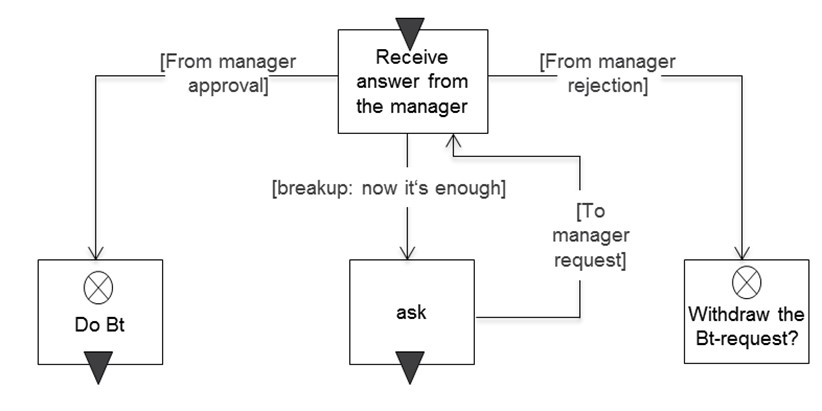
\includegraphics[width=0.7\linewidth]{20181026-Ontologie-Bilder/Grafiken-Ontologie/SUbjectExecution/ReceiveStateBreak}
	\caption[Message reception with manual interrupt]{Message reception with manual interrupt}
	\label{fig:receivestatebreak}
\end{figure}
\newpage

\subsection{Subject Behavior}
The possible sequences of a subject’s actions in a process are termed subject behavior. States and state transitions describe what actions a subject performs and how they are interdependent. In addition to the communication for sending and receiving, a subject also performs so-called internal actions or functions.

States of a subject are therefore distinct: There are actions on the one hand, and communication states to interact with other subjects (receive and send) on the other. This results in three different types of states of a subject. Figure \ref{fig:behavior-symbole} shows the different types of states with the coresponding symbols.

\begin{figure}[ph]
	\centering
	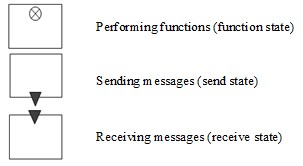
\includegraphics[width=0.5\linewidth]{20181026-Ontologie-Bilder/Grafiken-Ontologie/SUbjectExecution/Behavior-Symbole}
	\caption[State types and coresponding symbols]{State types and coresponding symbols}
	\label{fig:behavior-symbole}
\end{figure}

In S-BPM, work performers are equipped with elementary tasks to model their work procedures: sending and receiving messages and immediate accomplishment of a task (function state).
In case an action associated with a state (send, receive, do) is possible, it will be executed, and a state transition to the next state occurs. The transition is characterized through the result of the action of the state under consideration: For a send state, it is determined by the state transition to which subject what information is sent. For a receive state, it becomes evident in this way from what subject it receives which information. For a function state, the state transition describes the result of the action, e.g., that the change of a business object was successful or could not be executed.

The behavior of subjects is represented by modelers using Subject Behavior Diagrams (SBD). Figure \ref{fig:vollst-beispiel} shows the subject behavior diagram depicting the behavior of the subjects ‘employee’, ‘manager’, and ‘travel office’, including the associated states and state transitions. 

\begin{landscape}
\begin{figure}[ph]
	\centering
	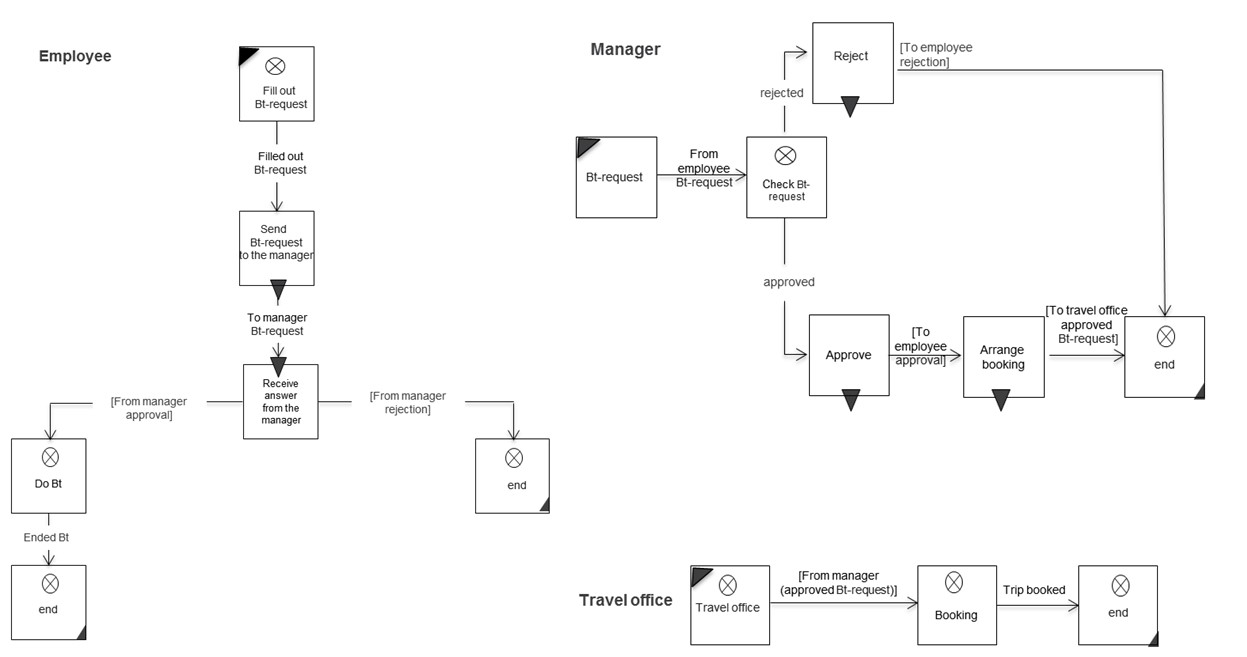
\includegraphics[width=0.7\linewidth]{20181026-Ontologie-Bilder/Grafiken-Ontologie/SUbjectExecution/Vollst-Beispiel}
	\caption[Subject behavior diagram for the subjects ‘employee’, ‘manager’, and ‘travel office’]{Subject behavior diagram for the subjects ‘employee’, ‘manager’, and ‘travel office’}
	\label{fig:vollst-beispiel}
\end{figure}
\end{landscape}
\newpage



\section{Ontology of Subject Behavior Description}

\begin{landscape}
\begin{figure}[ph]
	\centering
	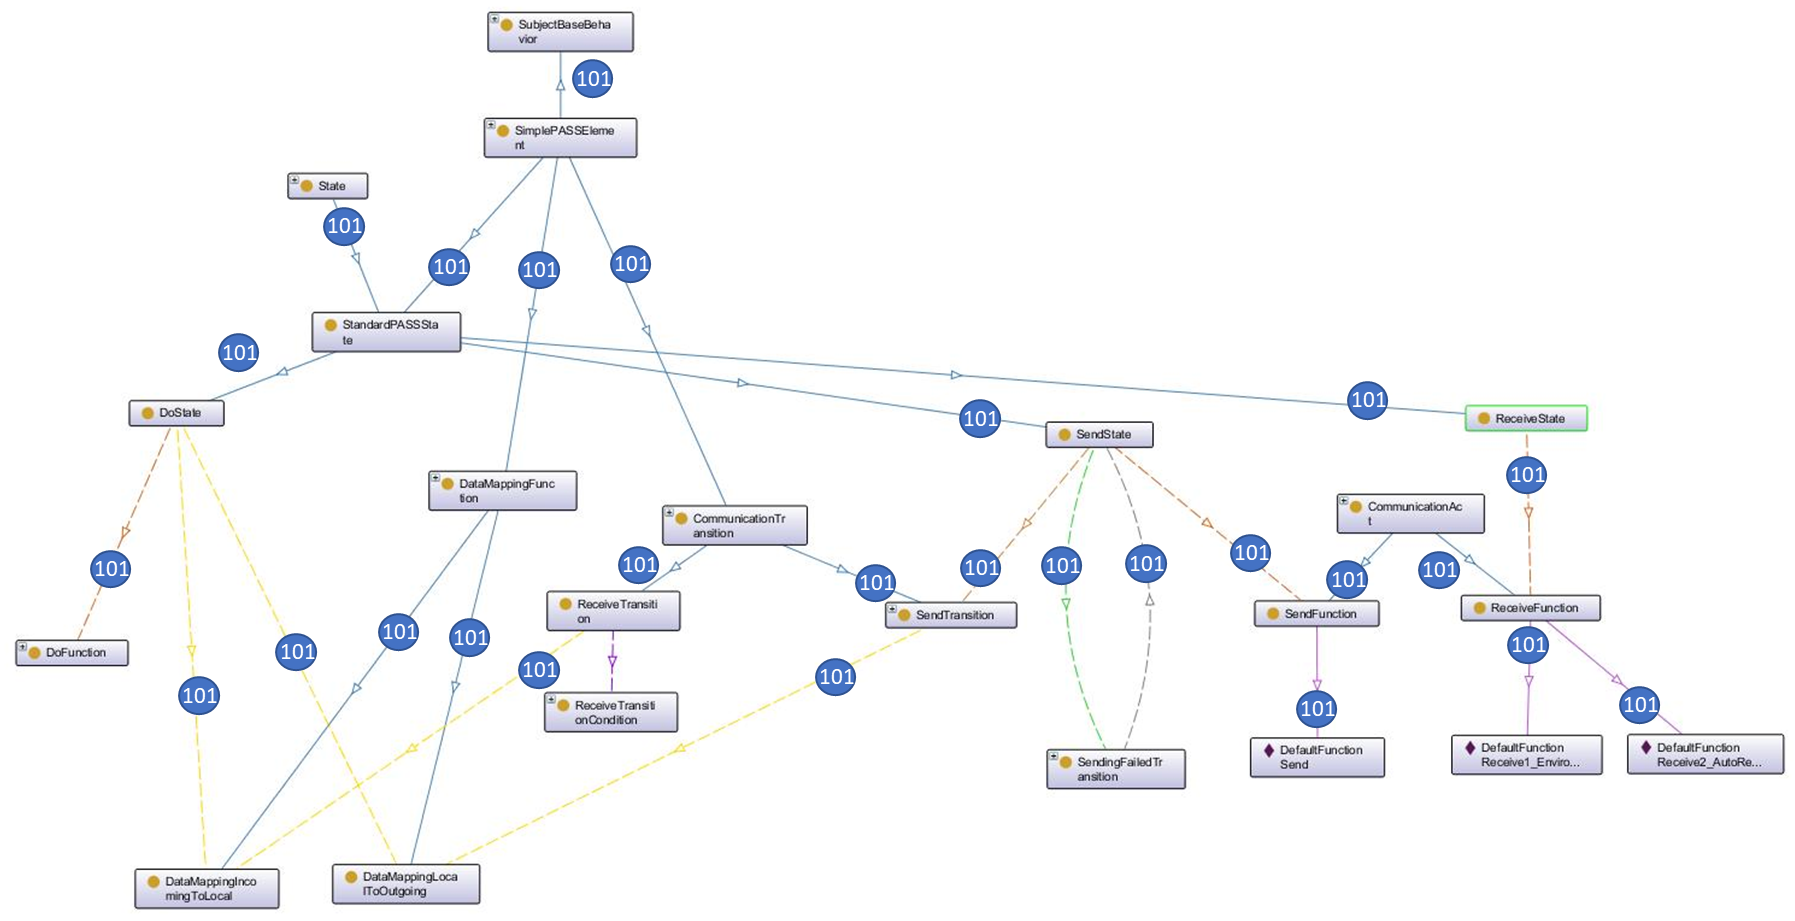
\includegraphics[width=1.0\linewidth]{20181026-Ontologie-Bilder/Grafiken-Ontologie/SUbjectExecution/20181218-SubjectBehavior}
	\caption[Behavior of subjects]{Behavior of subjects}
	\label{fig:20181218-subjectbehavior}
\end{figure}
\end{landscape}


\section{ASM Definition of Subject Execution}